In fully actuated systems, it is possible to produce a control scheme which asymptotically drives the deviations from some specified time-dependent trajectory to zero. This may be interpreted as defining an \textit{output function}, $h(q,t)$, with rank($h$) $= m$, which is identically zero when the trajectory is perfectly regulated, and attempting to maintain $h(q,t) = 0$. In underactuated systems, an output function may be defined, however since rank($h$) $<$ rank($q$), $h = 0$ defines a set of admissible values of $q$. In systems modelled by ordinary differential equations, the maximal internal dynamics of the system under the constraint $h=0$ is called the \textit{zero dynamics} \cite{isidori1995nonlinear}. It is possible to explicitly define the zero dynamics by synchronising all of the generalised coordinates of the system to a single variable labelled the \textit{phase variable}. The remaining variables are said to be under \textit{virtual constraints (VCs)}. %
\nomenclature{$\theta$}{The \textit{phase variable} to which all coordinates are synchronised in a virtual constraint} %
\nomenclature{VC}{Virtual (holonomic) constraint}

Walking robots are able to be modelled using ordinary differential equations for the majority of their motion, with the exception of their impact dynamics. We therefore apply virtual constraints over what are labelled the \textit{swing phases}, interspersed with impacts. The swing phase dynamics of the robot coupled with the applied virtual constraints, along with the impact dynamics, produce the \textit{hybrid zero dynamics} of the underactuated walker. In this section, we the derivation of hybrid zero dynamics for general underactuation degree one robots along with some useful results for the motion planner.
\nomenclature{HZD}{Hybrid zero dynamics}

\subsection{Dynamics of a general underactuated walker}
The general equation of motion of a nonlinear time-invariant physical system may be written as \cite{??}:
\begin{equation}\label{eqn:dynamics}
	M\left(q(t)\right)\ddot{q}(t) + C\left(q(t),\dot{q}(t)\right)\dot{q}(t)
	 + G\left(q(t)\right) = B\left(q(t)\right)u(t)
\end{equation}
where $M\left(q(t)\right)$ is the matrix of inertial terms, $C\left(q(t),\dot{q}(t)\right)$ is the matrix of Coriolis and centrifugal terms, $G\left(q(t)\right)$ is the gradient of the potential field and $B\left(q(t)\right)$ is some matrix which specifies the effect of control inputs $u(t)$. 

We model the dynamics of the walking robot by assuming that between each impact event, one leg, the \textit{stance leg} is pinned at its end. During the swing phase, the configuration of the robot evolves from $q^+$ immediately post-impact to $q^-$ immediately before the next impact. The other leg, the \textit{swing leg} interacts with the ground only upon impact, in which the swing leg instantaneously becomes the stance leg. This has several corollaries:
\begin{enumerate}[parsep=0cm]
	\item The forces at impact are impulsive and alter the velocities instantaneously but do not affect configurations.
	\item The collisions are purely inelastic, i.e. the swing leg becomes the stance leg without bouncing
	\item The stance leg lifts off the ground without further interaction; other than at the instant of impact, there is no time when both legs are in contact with the ground.
\end{enumerate}
Furthermore, we assume that all impacts occur without slipping. That is, the impulsive forces which occur at impact lie within the static friction cone. 

These assumptions represent an adequate model of physical walking and are widely used and discussed in the literature, see \cite{hurmuzlu1994rigid, westervelt2007feedback}. Under this impact model, there exists an impact map of following form \cite{manchester13planning}:
\begin{subequations}
\begin{align}
	q\left(t^+\right) &= Rq\left(t^-\right) \label{eqn:impactconfig}\\
	\dot{q}\left(t^+\right) &= R\Delta\left(q\left(t^-\right)\right)\dot{q}\left(t^-\right) \label{eqn:impactvel}
\end{align}
\end{subequations}

For the underactuated walkers considered in this thesis, $R$ represents a relabelling of coordinates. A simple example of relabelling of the coordinates at impact for a compass-gait walker is shown in Figure~\ref{fig:relabelimpact}.

\begin{figure}[htp]
\centering
\begin{minipage}{0.45\linewidth}
\centering
	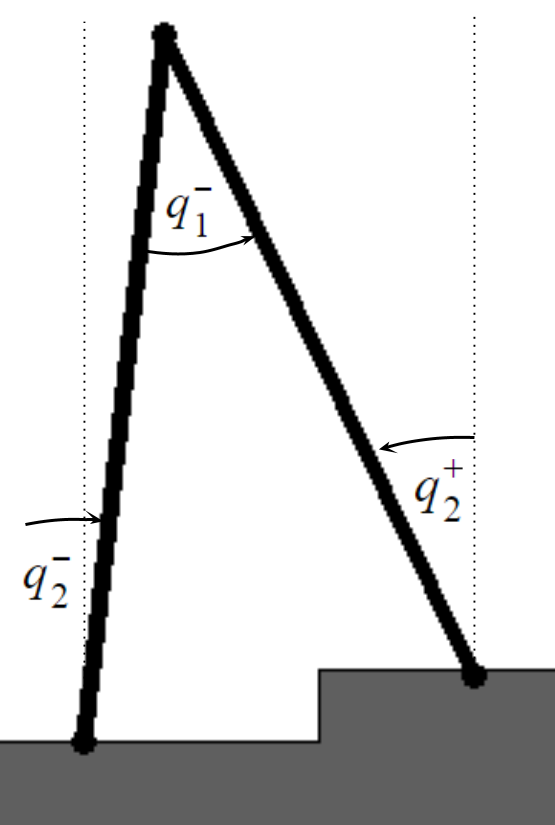
\includegraphics[width=0.7\linewidth]{3TechBackground/impact.png}
	\caption{Change of coordinates at impact for a compass-gait walker}
	\label{fig:relabelimpact}
\end{minipage}
\hspace{0.5cm}
\begin{minipage}{0.45\linewidth}
\begin{align*}
	q_1^+ &= -q_1^- \\
	q_2^+ &= -q_1^- + q_2 \\
	R &= \begin{bmatrix}
		-1	& 	0	\\
		-1	&	1
	\end{bmatrix}
\end{align*}
\end{minipage}
\end{figure}

To simplify the simulations and mathematics somewhat with no loss to in-principle generality of the method, all ground is considered to be piecewise flat. This implies that the normal force is always purely vertical and the frictional force is purely horizontal.

\subsection{Zero dynamics}
The application of virtual holonomic constraints synchronises a system's generalised coordinates to a single \textit{phase variable} $\theta$ which is increasing over the interval $[\theta^+, \theta^-]$. This produces functions of the following form: %
\nomenclature{$\theta^+$}{Value of phase variable just after impact} %
\nomenclature{$\theta^-$}{Value of phase variable just before impact}
\begin{subequations}
\label{eqn:virtconstraint}
\begin{align}
	q_i(t) &= \phi_i\left(\theta\right), &i = 1,2,\ldots,n \\
	\dot{q}_i(t) &= \frac{\partial\phi_i\left(\theta\right)}{\partial\theta}\dot{\theta}, &i = 1,2,\ldots,n \\
	\ddot{q}_i(t) &= \frac{\partial^2\phi_i\left(\theta\right)}{\partial\theta^2}\dot{\theta}^2 + \frac{\partial\phi_i\left(\theta\right)}{\partial\theta}\ddot{\theta}, &i = 1,2,\ldots,n
\end{align}
\end{subequations}
We define the following vector functions:
\begin{align*}
	\Phi\left(\theta\right) &= \left[ \phi_1\left(\theta\right), \phi_2\left(\theta\right), \ldots,
	\phi_n\left(\theta\right)\right]^T \\
	\Phi'\left(\theta\right) &= \left[ \frac{\partial\phi_1\left(\theta\right)}{\partial\theta},
	\frac{\partial\phi_2\left(\theta\right)}{\partial\theta}, \ldots ,
	\frac{\partial\phi_n\left(\theta\right)}{\partial\theta} \right]^T \\
	\Phi''\left(\theta\right) &= \left[ \frac{\partial^2\phi_1\left(\theta\right)}{\partial\theta^2},
	\frac{\partial^2\phi_2\left(\theta\right)}{\partial\theta^2}, \ldots ,
	\frac{\partial^2\phi_n\left(\theta\right)}{\partial\theta^2} \right]^T
\end{align*} %
\nomenclature{$\Phi\left(\theta\right)$}{Vector function describing the synchronisation of the generalised coordinates to the phase variable under a VC, i.e. $q=\Phi\left(\theta\right)$, $\dot{q} = \Phi'\left(\theta\right)\dot{\theta}$, etc}

Under the assumption perfect regulation of the virtual constraints, we can evaluate the zero dynamics by simple substitution into Equation~\ref{eqn:dynamics}:
\begin{equation*}
	M\left(\Phi(\theta)\right)\left[\Phi'(\theta)\ddot{\theta} + \Phi''\dot{\theta}^2\right] + 
	C\left(\Phi(\theta),\Phi'(\theta)\dot{\theta}\right)\Phi'(\theta)\dot{\theta} +
	G\left(\Phi(\theta)\right) = B\left(\Phi(\theta)\right)u_\alpha
\end{equation*}\nomenclature{$u_\alpha$}{Control which achieves perfect regulation of virtual constraint $\alpha$}%
where $u_\alpha$ is the control which achieves perfect regulation of the constraints. This may be rearranged into a more convenient form:
\begin{equation} \label{eqn:zerodyn}
	\alpha(\theta)\ddot{\theta} + \beta(\theta)\dot{\theta}^2 + \gamma(\theta) = 0
\end{equation}
where, if we denote $B^{\perp}(q)$ as a row vector which satisfies $B^{\perp}(q)B(q)u_\alpha = 0$,
\addtocounter{equation}{-1}
\begin{subequations}
\begin{align}
	\alpha(\theta) &= B^{\bot}\left(\Phi(\theta)\right)M\left(\Phi(\theta)\right)\Phi'(\theta) \\
	\beta(\theta) &= B^{\bot}\left(\Phi(\theta)\right)\left(M\left(\Phi(\theta)\right)\Phi''(\theta)
		+C\left(\Phi(\theta),\Phi'(\theta)\right)\Phi'(\theta) \right) \\
	\gamma(\theta) &= B^{\bot}\left(\Phi(\theta)\right)G\left(\Phi(\theta)\right)
\end{align}
\end{subequations}

\subsection{Partial closed-form solutions for velocity and energy}
One of the useful properties of virtual constraints is that they allow precomputation of a partial closed-form solution for velocity and energy. The solution is partial in that we obtain an expression for $\dot{\theta}^2$ in terms of $\theta$ rather than time. Under the assumption that $\theta$ is monotonic, it can be used as a new dependent variable:
\begin{align*}
	\frac{d}{d\theta}\left[\dot{\theta}\left(t(\theta)\right)^2\right] &= 
	\frac{d}{dt}\frac{dt}{d\theta}\left[\frac{d\theta}{dt}\left(t(\theta)\right)^2\right] \nonumber \\ 
	&= 2\ddot{\theta}\left(t(\theta)\right)
\end{align*}
Substituting Equation~\ref{eqn:zerodyn} into this expression, we arrive at a first-order ODE in $\dot{\theta}(\theta)^2$:
\begin{equation}\label{eqn:zerodynDE}
	\frac{d}{d\theta}\dot{\theta}(\theta)^2 = -2\frac{\beta(\theta)}{\alpha(\theta)}
		\dot{\theta}(\theta)^2 - 2\frac{\gamma(\theta)}{\alpha(\theta)}
\end{equation}
If we assume, as in \cite{manchester13planning}, that for all $\theta \in [\theta^+, \theta^-]$, we have local instantaneous controllability, i.e. $\alpha(\theta) \neq 0$, then we may solve Equation~\ref{eqn:zerodynDE} numerically over $[\theta^+, \theta^-]$, which yields an affine solution, i.e.
\begin{equation} \label{eqn:affinesoln}
	\dot{\theta}(\theta)^2 = \Gamma(\theta)\dot{\theta}^{+^2} + \Psi(\theta)
\end{equation}

For typical walking motions, there exits a single point of maximum potential energy within each footstep. This corresponds to a zero crossing of $\gamma(\theta)$. If we denote the velocity at this point the \textit{critical velocity}, $\dot{\theta}(\theta_c)$, the affine form of Equation \ref{eqn:affinesoln} allows us to trivially determine the feasibility of a particular constraint given the initial velocity; for any given constraint there exists an initial velocity which satisfies
\begin{equation} \label{eqn:critvel}
	\Gamma(\theta_c)\dot{\theta}^{+^2}_c + \Psi(\theta_c) = 0
\end{equation}
For any initial velocity less than $\dot{\theta}^+_c$, there is no real solution for Equation \ref{eqn:affinesoln} at $\theta_c$; the robot will fall back rather than complete the footstep.

Following from Equation \ref{eqn:affinesoln}, we may also derive the total mechanical energy of the system. For general systems with dynamics as expressed in Equation~\ref{eqn:dynamics}, the mechanical energy has the form:
\[ H\left(q,\dot{q}\right) = \dot{q}^TM(q)\dot{q} + V(q) \]
Under perfectly regulated virtual constraints, this reduces to:
\begin{align*}
	H\left(\theta,\dot{\theta}\right) &= \Upsilon(\theta)\dot{\theta}^2+\Xi(\theta) \\
	\Upsilon(\theta) &= \Phi'(\theta)^TM\left(\Phi(\theta)\right)\Phi'(\theta) \\
	\Xi(\theta) &= V\left(\Phi(\theta)\right)
\end{align*}
Since this is affine in $\dot{\theta}^2$ for a given $\theta$, we may trivially calculate the closed form:
\begin{equation}
	H\left(\theta, \dot{\theta}_0^2\right) =
	\Upsilon(\theta)\Gamma\left(\theta\right)\dot{\theta}_0^2 +
	\Upsilon(\theta)\Psi\left(\theta\right) + \Xi(\theta)
\end{equation}

\subsection{Impact conditions} \label{sec:impact}
It is not possible to apply virtual constraints across impacts since the dynamics of impact are discontinuous; the impulsive forces applied by the ground on the end of the swing leg occur over too short a time period to oppose through the application of control. The dynamics of impact from Equations \ref{eqn:impactconfig} and \ref{eqn:impactvel} are therefore independent of the control applied over the swing phases. 

In order to be admissible, a virtual constraint must satisfy the following conditions. Consider $\alpha$ to denote the constraint which precedes $\beta$:
\begin{samepage}
\begin{adjustwidth}{1.8cm}{}
\begin{enumerate}[label=\bfseries Condition \arabic*, parsep=0pt]
	\item $\Phi_\beta\left(\theta_\beta^+\right) = R\Phi_\alpha\left(\theta_\alpha^-\right)$ -- The initial configuration of the constraint matches the output of the impact map for the final configuration of the previous constraint. \label{item:configinvariance}
	\item $\Phi_\beta'\left(\theta_\beta^+\right)\dot{\theta}^+ = R\Delta\left(\Phi_\alpha(\theta_\alpha^-)\right)\Phi_\alpha'\left(\theta_\alpha^-\right)\dot{\theta}^-$ -- The initial velocity under the constraint matches the the post-impact velocity following the previous constraint. \label{item:velinvariance}
	\item The vertical component of the post-impact velocity of the end of the new swing leg, $\dot{p}_v^+ > 0$ -- The new swing lifts off the ground immediately after impact. \label{item:liftoff}
	\item $F_N > 0$ -- the vertical force at impact is compressive; the ground resists the leg rather than attracts it. \label{item:posnormalF}
	\item $|F_T|/F_N<\mu_s$ -- the forces at impact lie within the friction cone. \label{item:frictioncone}
\end{enumerate}
\end{adjustwidth}
\end{samepage}

\ref{item:configinvariance} and \ref{item:velinvariance} refer to what may be labelled the \textit{invariance of the zero dynamics}; they specify the requirement of a constraint to match the previous constraint in configuration and velocity through the impact map. The remaining conditions must be met in order for the assumptions made about the impact map to be reasonable.

\subsection{B{\'e}zier curves as virtual constraints} \label{sec:bezconstraints}
Bézier curves provide a way to produce families of curves for particular start and end heights and are sparsely identified by only $N+1$ points, where $N$ is the degree of the curve. These points provide an intuitive way of defining the curve, in contrast with polynomial coefficients. Furthermore, as demonstrated in \cite{westervelt2007feedback}, the use of Bézier polynomials to describe the virtual constraint leads to a closed form of the invariance conditions described in Section \ref{sec:impact}. 

A general Bézier curve is defined by the following parametric equation.
\begin{equation}
	\begin{bmatrix}
		\theta \\ b_k
	\end{bmatrix}
	=
	\sum_{i=0}^{N}\binom{N}{i}\left(1-t\right)^{N-i}t^i
	\begin{bmatrix}
		\theta_i \\ \alpha^k_i
	\end{bmatrix} \label{eqn:genBez}
\end{equation}
Since this equation is not monotonic in $\theta$, it is not a convenient expression. Therefore, we build families of Bézier curves with the following formulation.
\begin{subequations} \label{eqn:usefulBez}
\begin{align}
	t &= \frac{\theta - \theta^+}{\theta^- - \theta^+} \\
	b_k &= \sum_{i=0}^{N}\binom{N}{i}\left(1-t\right)^{N-i}t^i~\alpha^k_i
\end{align}
\end{subequations}
%This is expressible explicitly as
%\begin{equation}
%	b_k = \frac{1}{\left(\theta_N - \theta_0\right)^N}\sum_{i=0}^{N}\binom{N}{i}
%		\left(\theta_N - \theta\right)^{N-i}
%		\left(\theta - \theta_0\right)^i~\alpha^k_i \label{eqn:expBez}
%\end{equation}
This formulation produces curves of the form given in Equation~\ref{eqn:genBez} with
\[\theta_i = \frac{i}{N}\left(\theta^- - \theta^+\right) + \theta+ ~~
	\forall ~~ i \in \left[1,~N-1\right]\]

The use of Bézier polynomials in this manner to define constraints trivially generalises to arbitrary dimensions. We define the output function to be:
\begin{subequations}\label{eqn:outputfun} 
\begin{align} 
	h_\alpha(q) &:= H_0 q - B_\alpha \circ \theta(q) \\
	\theta(q) &= cq \\
	H &= \begin{bmatrix}
		H_0 \\ c
	\end{bmatrix}
\end{align}
\end{subequations}
Where $\theta(q)$ is the phase variable, each row of $B_\alpha\circ\theta(q)$ is a Bézier polynomial of the form of Equation \ref{eqn:usefulBez}, $c$ is a $1\times n$ vector and $H_0$ is a $(n-1)\times n$ matrix.

This avails a convenient and compact method to encapsulate the parameters of the virtual constraints; each row of Equation \ref{eqn:outputfun} is a Bézier polynomial with coefficients $\alpha_1^k, \ldots, \alpha_N^k$, so all coefficients may be stored in a $(n-1)\times(N+1)$ matrix $\alpha$. For notational convenience, we define each column of $\alpha$ by $\alpha_i := [\alpha_i^1; \ldots; \alpha_i^{n-1}]$. %
\nomenclature{$\alpha$}{Matrix of Bézier coefficients defining a virtual constraint; $\alpha_i$ is a column of $\alpha$}

A characteristic property of Bézier polynomials is that the value of $b_k$ and its derivative at the endpoints are explicitly set by the coefficients:
\begin{subequations}
\begin{align}
	\Phi_\alpha\left(\theta_\alpha^+\right) &= H^{-1}\begin{bmatrix}
		\alpha_0 \\ \theta_\alpha^+
	\end{bmatrix} \\
	\Phi_\alpha\left(\theta_\alpha^-\right) &= H^{-1}\begin{bmatrix}
		\alpha_N \\ \theta_\alpha^-
	\end{bmatrix} \\
	\Phi_\alpha'\left(\theta_\alpha^+\right) &= H^{-1}\begin{bmatrix}
		\frac{N}{\theta_\alpha^- - \theta_\alpha^+}(\alpha_1 - \alpha_0) \\
		1
	\end{bmatrix} \\
	\Phi_\alpha'\left(\theta_\alpha^-\right) &= H^{-1}\begin{bmatrix}
		\frac{N}{\theta_\alpha^- - \theta_\alpha^+}(\alpha_N - \alpha_{N-1}) \\
		1
	\end{bmatrix}
\end{align}
\end{subequations}

The invariance conditions, \ref{item:configinvariance} and \ref{item:velinvariance} in Section \ref{sec:impact}, can be written in closed form \cite{westervelt2007feedback}, with $\beta$ being the constraint following $\alpha$:

\begin{equation} \label{eqn:bezinvconfig}
	\begin{bmatrix}
	 \beta_0 \\ \theta_\beta^+
	\end{bmatrix}
	= HRH^{-1} \begin{bmatrix}
		\alpha_N \\ \theta_\alpha^-
	\end{bmatrix} \\
\end{equation}
\begin{subequations} \label{eqn:bezinvvel}
\begin{align}
	\beta_1 &= \frac{\theta_\beta^- - \theta_\beta^+}{N_\beta}
	H_0\Delta_{\dot{\theta}_\alpha} \left(c\Delta_{\dot{\theta}_\alpha}\right)^{-1} + \beta_0\\
	\Delta_{\dot{\theta}_\alpha} &= R\Delta\left(\Phi_\alpha\left(\theta_\alpha^-\right)\right)
		\Phi_\alpha'\left(\theta_\alpha^-\right) \label{eqn:Delthd}
\end{align}
\end{subequations}

Imposing the invariance conditions constrains the coefficients $\beta_0$ and $\beta_1$ to be functions of $\alpha_N$ and $\alpha_{N-1}$. In order for this to make sense in the context of continuous walking, this implies that the minimum degree of Bézier polynomial chosen to define each constraint must be no less than 3.

For any given robot, the position $p=[p_h;p_v]$ of the end of the swing leg is a function of the generalised coordinates. If the robot operates under a set of virtual constraints of the form of Equation \ref{eqn:virtconstraint}, then %
\nomenclature{$p$}{The position of the end of the swing leg, $p = [p_h;p_v]$}
\begin{equation*}
	\dot{p} = \frac{\partial p\Big(\Phi(\theta)\Big)}{\partial\Phi(\theta)}
	\Phi'(\theta)\dot{\theta}
\end{equation*}

By hypothesis, $\theta$ is increasing, so \ref{item:liftoff} is satisfied if Equation \ref{eqn:liftoff} is true for the constraint $\alpha$.
\begin{equation} \label{eqn:liftoff}
	[0~1]~\frac{\partial p}{\partial\Phi_\alpha(\theta)}
	\left(\Phi_\alpha\left(\theta_\alpha^+\right)\right)\Phi_\alpha'\left(\theta_\alpha^+\right)>0
\end{equation}
Note that since $\Phi\left(\theta^+\right)$ and $\Phi'\left(\theta^+\right)$ are fixed by the invariance condition on the basis of the previous constraint, in order for the constraint $\alpha$ to be useful, the final state under $\alpha$ must allow for a constraint which satisfies invariance following $\alpha$ to also satisfy \ref{item:liftoff}. That is:
\begin{equation} \label{eqn:liftoffNext}
	[0~1]~\frac{\partial p}{\partial\left(R\Phi_\alpha(\theta)\right)}
	\left(R\Phi_\alpha\left(\theta_\alpha^-\right)\right)
	R\Delta\left(\Phi_\alpha\left(\theta_\alpha^-\right)\right)
	\Phi_\alpha'\left(\theta_\alpha^-\right)>0
\end{equation}

Similarly, \ref{item:posnormalF} is satisfied if $\dot{p}_v^- < 0$, therefore it is satisfied if
\begin{equation} \label{eqn:posnormalF}
	[0~1]~\frac{\partial p}{\partial\Phi_\alpha(\theta)}
	\left(\Phi_\alpha\left(\theta_\alpha^-\right)\right)\Phi_\alpha'\left(\theta_\alpha^-\right)<0
\end{equation}

It is possible to write the force at impact in the following manner, with $F = [F_T;F_N]$ \cite{westervelt2007feedback}:
\[ F = \Delta_{F}(q^-)\dot{q}^- \]
Therefore \ref{item:frictioncone} is satisfied if 
\begin{equation}
	\left\lvert\frac{[1~0]~\Delta_F(\Phi_\alpha\left(\theta_\alpha^-\right)) \Phi_\alpha'\left(\theta_\alpha^-\right)}
		{[0~1]~\Delta_F(\Phi_\alpha\left(\theta_\alpha^-\right)) \Phi_\alpha'\left(\theta_\alpha^-\right)}\right\rvert
		< \mu_s
\end{equation}